\documentclass[15pt]{article}

\usepackage{amsfonts} % To do stylized R and stuff
\usepackage{amsmath}  % For the question* enviroment
\usepackage{indentfirst} % Adds an indent after the section thing

% Plot stuff
\usepackage{tikz}
\usepackage{pgfplots}
\pgfplotsset{compat=1.18} % Use the latest version you have

% Psuedocode
\usepackage{algorithm}
\usepackage{algpseudocode}
\usepackage{float} % To avoid the algorithms floating around

% Margin - 1 inch on all sides
\usepackage[letterpaper]{geometry}
\usepackage{times}
\geometry{top=1.0in, bottom=1.0in, left=1.0in, right=1.0in}

% Add space between paragraphs
\setlength{\parskip}{0.5em} % or another value like 0.5em or 10pt

%
% Doublespacing
%
% \usepackage{setspace}
% \doublespacing        % I am not going to use this here but it is good to
                        % know about

%
% Rotating tables (e.g. sideways when too long)
%
\usepackage{rotating}

%
% Fancy-header package to modify header/page numbering (insert last name)
%
\usepackage{fancyhdr}
\pagestyle{fancy}
\lhead{}            % Makes the left header empty
\chead{}            % Makes the center header empty
\rhead{\thepage}    % Puts a page number of the right header
\lfoot{}            % Makes left footer empty
\cfoot{}            % Makes center footer empty
\rfoot{}            % Makes right footer empty
\renewcommand{\headrulewidth}{0pt}  % Removes the horizontal line under the 
                                    % header.
\renewcommand{\footrulewidth}{0pt}  % Removes the horizontal line above the 
                                    % footer.
%To make sure we actually have header 0.5in away from top edge
%12pt is one-sixth of an inch. Subtract this from 0.5in to get headsep value
\setlength\headsep{0.333in}

%
% Makes it so that section numbers are bold, but not the text
%
\usepackage{titlesec}
\titleformat{\section}
  {\large}                  % Smaller than default \Large
  {\bfseries\thesection}    % Bold number
  {1em}
  {}

%%%%%%%%%%%%%%%%%
% Begin document
%%%%%%%%%%%%%%%%%
\begin{document}
\begin{flushleft}

%Title
\begin{center}
    \bfseries\LARGE Course Project: Cryptographic Algorithms \& 
                    ModularArithmetic \\
    \bfseries\Large Shamir’s Secret Sharing \\
    \bfseries\large By Diego Martinez
\end{center}

%Changes paragraph indentation to 0.5in
\setlength{\parindent}{0.5in}
%Begin body of paper here

\section{\textbf{Shamir's Secret Sharing and it's purpose}}
Shamir's Secret Sharing (SSS) algorithm is an encryption algorithm that takes a
secret, and split it into different pieces or, in other words, shares with the
number of shares is denoted by $N$. The secret can only be reconstructed if 
there is enough shares, or meet the threshold of shares, which is denoted by a
number $K$.

Basically, a secret can be split among different people, and those people can
only reconstruct the secret if enough people agree to recreate it.

How it can be implemented, polynomials would be used to create the shares and
also recreate the secret. Lets say a polynomial $y = ax + b$. The $b$ in this
case is the constant, and for SSS it would be the secret that is to be
encrypted. Shares would be made by plugging in random numbers of $x$ and finding
the $y$, and that pair $(x,y)$ would be a share. The coefficient(s) can be any
random number when creating shares. For decrypting a secret, the polynomial that
goes through $K$ points must be found, and again the constant of that polynomial
would be the secret. Using the modulus can also be used in SSS, but will be
covered later.

\section{\textbf{Mathematical background}}
In order to implement SSS, there are some concepts to go over first. The first
which is the \textbf{Lagrange Polynomial Interpolation}, which is used to find the
polynomial of the lowest degree that goes through all of the shares. A Lagrange
polynomial of some share's $x$ coordinate $x_i$, is a polynomial that its $y$
value at that $x_i$ is $1$, and is $0$ for every other share's, at least the
shares inputted, $x$ coordinate.

For example, lets say there are some $x$ coordinates $x=1,2,3,4$, the Lagrange
equation of the $x$ coordinate $2$, would be some polynomial such that $f(2)=1$,
and $f(1)=f(3)=f(4)=0$

After getting the polynomial for that value of $x_i$, the polynomial would be
multiplied by the $x_i$'s respective $y$ value, and now there would be an
equation that still is $0$ at all other share's $x$ value, but now goes through
the $x_i$'s share. The same thing will be done for all other shares, where the
the Lagrange polynomial for those shares are found, and multiply by their 
respective $y$ values. After getting all of these Lagrange polynomials and add
them together, there would now be a polynomial that goes through all of the 
shares.

Here is the equations for Lagrange Polynomial Interpolation.
\begin{align*}
    l_{i}(x) = \prod_{j=0, j\neq i}^{n} \frac{x-x_{j}}{x_{i}-x_{j}} \\
    f(x) = \sum_{i=0}^{K-1} y_{i}l_{i}(x)
\end{align*}

Looking at the first line, there is a product operator ($\prod$). This means
that all of the fractions where the divisor is the value of $x_i$ who's Lagrange
equation is being found minus another share's $x$ value, and the dividend is
$x$ minus the same share's x value as is being subtracted in the divisor, and
all of those fractions are multiplied together.

For example, say that, again, there are some $x$ coordinates $x=1,2,3,4$, the
Lagrange equation of $x=2$ would be:
\begin{align*}
    l_2(x) = \frac{x-1}{2-1} \times \frac{x-3}{2-3} \times \frac{x-4}{2-4}
\end{align*}

Now looking at the second equation, this is the implementation of multiplying
each Lagrange polynomial by their respective $y$, then adding all Lagrange
polynomials to finally get the polynomial that goes through all the shares.

Walking through the full example of $x=1,2,3,4$, the follow Lagrange polynomials
are found:
\begin{align*}
    l_1(x) = \frac{x-2}{1-2} \times \frac{x-3}{1-3} \times \frac{x-4}{1-4} \\
    l_2(x) = \frac{x-1}{2-1} \times \frac{x-3}{2-3} \times \frac{x-4}{2-4} \\
    l_3(x) = \frac{x-1}{3-1} \times \frac{x-2}{3-2} \times \frac{x-4}{3-4} \\
    l_4(x) = \frac{x-1}{4-1} \times \frac{x-2}{4-2} \times \frac{x-3}{4-3}
\end{align*}
Now, multiplying each Lagrange polynomial by there respective $y$, let it be
$y=5,6,7,8$, then simplifying the equation, the following is found:
\begin{align*}
    f(x) = x + 4
\end{align*}
Plotting the line $f(x)=x+4$, it does indeed go thought the points $(1,5),(2,6),
(3,7),(4,8)$.
\begin{center}
\begin{tikzpicture}
\begin{axis}[
    axis lines = middle,
    xlabel = $x$,
    ylabel = $y$,
    grid = both,
    xmin = 0, xmax = 5,
    ymin = 0, ymax = 10,
    samples = 100
]
    % Plot the line f(x) = x + 4
    \addplot[domain=0:5, blue, thick]{x + 4};

    % Plot the points
    \addplot[only marks, red] coordinates {
        (1,5) (2,6) (3,7) (4,8)
    };
\end{axis}
\end{tikzpicture}
\end{center}

In the case of SSS, we would not use the variable $x$ at all like in the
equation $f(x)=x+4$. Instead, the values of each Lagrange polynomial at $x=0$
would be looked for, as the constant of the polynomial would be the secret. So
the new equations for the use of SSS would be:
\begin{align*}
    l_{i}(0) = \prod_{j=0, j\neq i}^{n} \frac{-x_{j}}{x_{i}-x_{j}} \\
    f(x) = \sum_{i=0}^{K-1} y_{i}l_{i}(0)
\end{align*}
The bottom equation would stay the same.

With just the Lagrange Polynomial Interpolation, a basic version of SSS can be
achieved, but another concept that could be added to improve the security of the
algorithm. This concept is \textbf{Modular Arithmetic}. Modular Arithmetic is
where the remainder of division. For example, the remainder of 8 divided by 6 is
2. Equivalently, $8 \bmod 6$ would be $2$. When applying this to an
equation, for example $(x+4) \bmod 7$ we get:
\begin{center}
\begin{tikzpicture}
\begin{axis}[
    axis lines = middle,
    xlabel = $x$,
    ylabel = $y$,
    grid = both,
    xmin = -1, xmax = 11,
    ymin = -1, ymax = 7.5,
    xtick = {0,1,2,3,4,5,6,7,8,9,10},
    ytick = {0,1,2,3,4,5,6,7},
    enlargelimits=0.1,
    legend style={at={(0.5,1.05)}, anchor=south}
]
\addplot[
    color=blue,
    thick,
    sharp plot
] table {
    x  y
    0  4
    1  5
    2  6
    3  7
};
\addplot[
    color=blue,
    thick,
    sharp plot
] table {
    x  y
    3  0
    4  1
    5  2
    6  3
    7  4
    8  5
    9  6
    10 7
};
\end{axis}
\end{tikzpicture}
\end{center}
Looking at this graph, we can see that the equation $y=x+4$ loops around under
the line $x=7$. How does this apply to the SSS algorithm? Now that we have a
polynomial with the secret of $4$  under the modulus of $7$ in this case, we
make some shares. Let $x=1,2,3,4$. Plug them into the polynomial and we get
$y=5,6,0,1$. Now the points look scrambled, and would be much harder to brute
force looking for a polynomial that contains the secret using Lagrange if there
are some shares known but not enough to recreate the secret. The divisor number
thing will be referred to as modulus in this report, like the number $7$ in
$\bmod 7$ will be referred to as modulus.

One more thing to note about doing $\bmod$ is that we cannot do regular division
under $\bmod$. For example, the fraction in $(\frac{3}{7}) \bmod 5$ cannot be
done regularly. The way around this is that we have to find the \textbf{mod
inverse} of the divisor. The $\bmod$ inverse of a number $a$ is a number $b$
under $\bmod c$ such that $b \cdot a \bmod c = 1$. For example, the $\bmod$
inverse of $7$ under $\bmod 5$ is $3$ since $3 \cdot 7 \bmod 5 = 1$. Now that we
have the $\bmod$ inverse, we can multiply the dividend by the $\bmod$ inverse
and that would be how we do division under $\bmod$. 

\section{\textbf{Pseudocode}}

Now how can we implement all of this? Let us first look at \textbf{encryption}.
To encrypt a secret, we need the number that we want to be a secret $S$, the
number of shares $N$, and the threshold $K$, making sure that $N \geq K$ since
we need enough shares to recreate the secret. The degree of polynomial needed to
encrypt the secret would be $K-1$, so for threshold of $3$, we would need a
second degree polynomial. for example $ax^2 + bx + c = y$. The coefficients can
be any random integer, but let us make sure that all of them are not $0$. The
secret would again be the constant $c$. Now to implement the $\bmod$ stuff, we
must choose a prime number to be the modulus to avoid any weirdness when doing
the $\bmod$ calculation. The modulus must also be greater than $S,K,N$. For
this report, we will choose the next biggest prime number of the greatest number
between the $S,K,N$. \textbf{Now lets get the steps for encryption}:
\begin{enumerate}
    \item Input the $S,K,N$, making sure that $N \geq K$
    \item Calculate what degree polynomial would be needed $(K-1)$
    \item Calculate modulus (a prime number $> S,K,N$)
    \item Populate the coefficient with random numbers less than modulus
    \item Create $N$ shares using the coefficients
    \item Output the shares and the calculated modulus
\end{enumerate}

% General encryption algorithm
\begin{algorithm}[H]
\caption{Encryption}
\begin{algorithmic}[1] % The [1] adds line numbers
\Statex \textbf{Input:} A value $S$ to encrypt, a value $K$ as a threshold, and
        a value $N$ as the number of shares wanted
\Statex \textbf{Output:} Calculated shares and modulus
\Function{generateY}{polynomial, $x$, modulus}
    \State $y:=$ polynomial[$0$]
    \For{i \textbf{to} (len(polynomial)-1)}
        \State $y := y + x^{i+1}$
    \EndFor
    \State \Return $y \bmod$ modulus
\EndFunction
\State
% End program if condition
\If{$K > N$}
    \State \textbf{End}
\EndIf
\State
\State degree $:= K-1$ 
\State
% Get the biggest number out of S,K,N and calculate modulus accordingly
\If{secret $\geq K$ \textbf{and} secret $\geq N$}
    \State tempMod $:=$ secret
\ElsIf{$K \geq $ secret \textbf{and} $K \geq N$}
    \State tempMod $:= K$
\Else
    \State tempMod $:= N$
\EndIf
\State modulus = \Call{greaterPrime}{tempMod}
\State polynomial $:=$ [$S$]
\For{$i:=0$ \textbf{to} degree}
    \State polynomial.append(randint($1,\text{modulus}-1$))
\EndFor
\State
\State shares = []
\For{$i:=0$ \textbf{to} $N$}
    \State point $:=$ []
    \State $x:=$ randint(1, $\mathbb{Z}$)
    \State $y:=$ \Call{generateY}{polynomial, $x$, modulus}
    \State point.append($x$)
    \State point.append($y$)
    \State shares.append(point)
\EndFor
\State \Return (shares, modulus)
\end{algorithmic}
\end{algorithm}
You see a function called GREATERPRIME was used in this Pseudocode, and it will
be defined later. In lines 2-11, we have a function that generates a $y$ value
given the polynomial coefficients, the $x$ value, and the modulus. By
multiplying each coefficient by $x$ to its respective power and adding the $y$
constant, or secret, we are able to generate $x$'s $y$ point, and that would be
one share, of course after taking the modulus of the $y$ to make sure that it is
in the field of $y$ values that our polynomial is in.

% Prime number functions
\begin{algorithm}[H]
\caption{Prime number functions}
\begin{algorithmic}[1]
% Function for to check if number is prime
\Function{prime}{$n$}
    \For{$i:=0 \textbf{ to } \sqrt{|n|}+1 $}
        \If{$n \bmod i = 0$}
            \State \Return \textbf{false}
        \EndIf
        \State \Return \textbf{true}
    \EndFor
\EndFunction
\State
% Function to calculate a prime number bigger than number
\Function{greaterprime}{number}
    \State{primeNumber $:=$ number $+1$}
    \While{\textbf{not} \Call{prime}{primeNumber}}
        \State primeNumber $:=$ primeNumber $+1$
    \EndWhile
    \State \Return primeNumber
\EndFunction
\end{algorithmic}
\end{algorithm}
Here we have how we can calculate our prime number for modulus. where we brute
force finding the prime number by continuously adding 1 to the given number
that number is prime. To the best of my knowledge, this is the best of finding
a prime number.

Lets move onto the fun part, \textbf{the decryption}. Note that the modulus must
be known to recreate the secret, as to my knowledge, there is no way to
calculate the modulus with just the shares. When it comes to mod, remember that
we cannot do regular division when under mod and that we would need to find the
mod inverse of the divisor then multiply it by the dividend. I am not sure if it
is correct, but it works for me, but after getting the Lagragne polynomial's
values at $x=0$, multiply by there respective $y$ values, then added them all
up, we have to do the mod of that final value. \textbf{Now lets go over the 
steps for decryption:}
\begin{enumerate}
    \item Input some number of shares and the modulus
    \item 
\end{enumerate}

\end{flushleft}
\end{document}